\subsection{Deep Neural Network (DNN)}\label{subsec:dnn}
A Deep Neural Network (DNN) is an artificial neural network that employs more than one hidden layer between the input and output layers to classify an input pattern or, more generally, learn to approximate a target function $f$. In the presence of a classification problem, such as the SI problem, an attempt is made to discriminate a pattern $x$ based on a feature $y$, which can take value among $Q$ categories (also called classes), and the DNN estimates the class probabilities $p_j, j \in \{1, ..., Q\}$. The input features to a DNN do not require special attention to preprocessing, and in fact in audio processing one can range from raw frames of audio, to MFCCs/MFCCs \& deltas, to Mel's log-scaled spectrogram features. Figure \vref{fig:dnn0} shows an example neural network for classification tasks.

\begin{figure}
	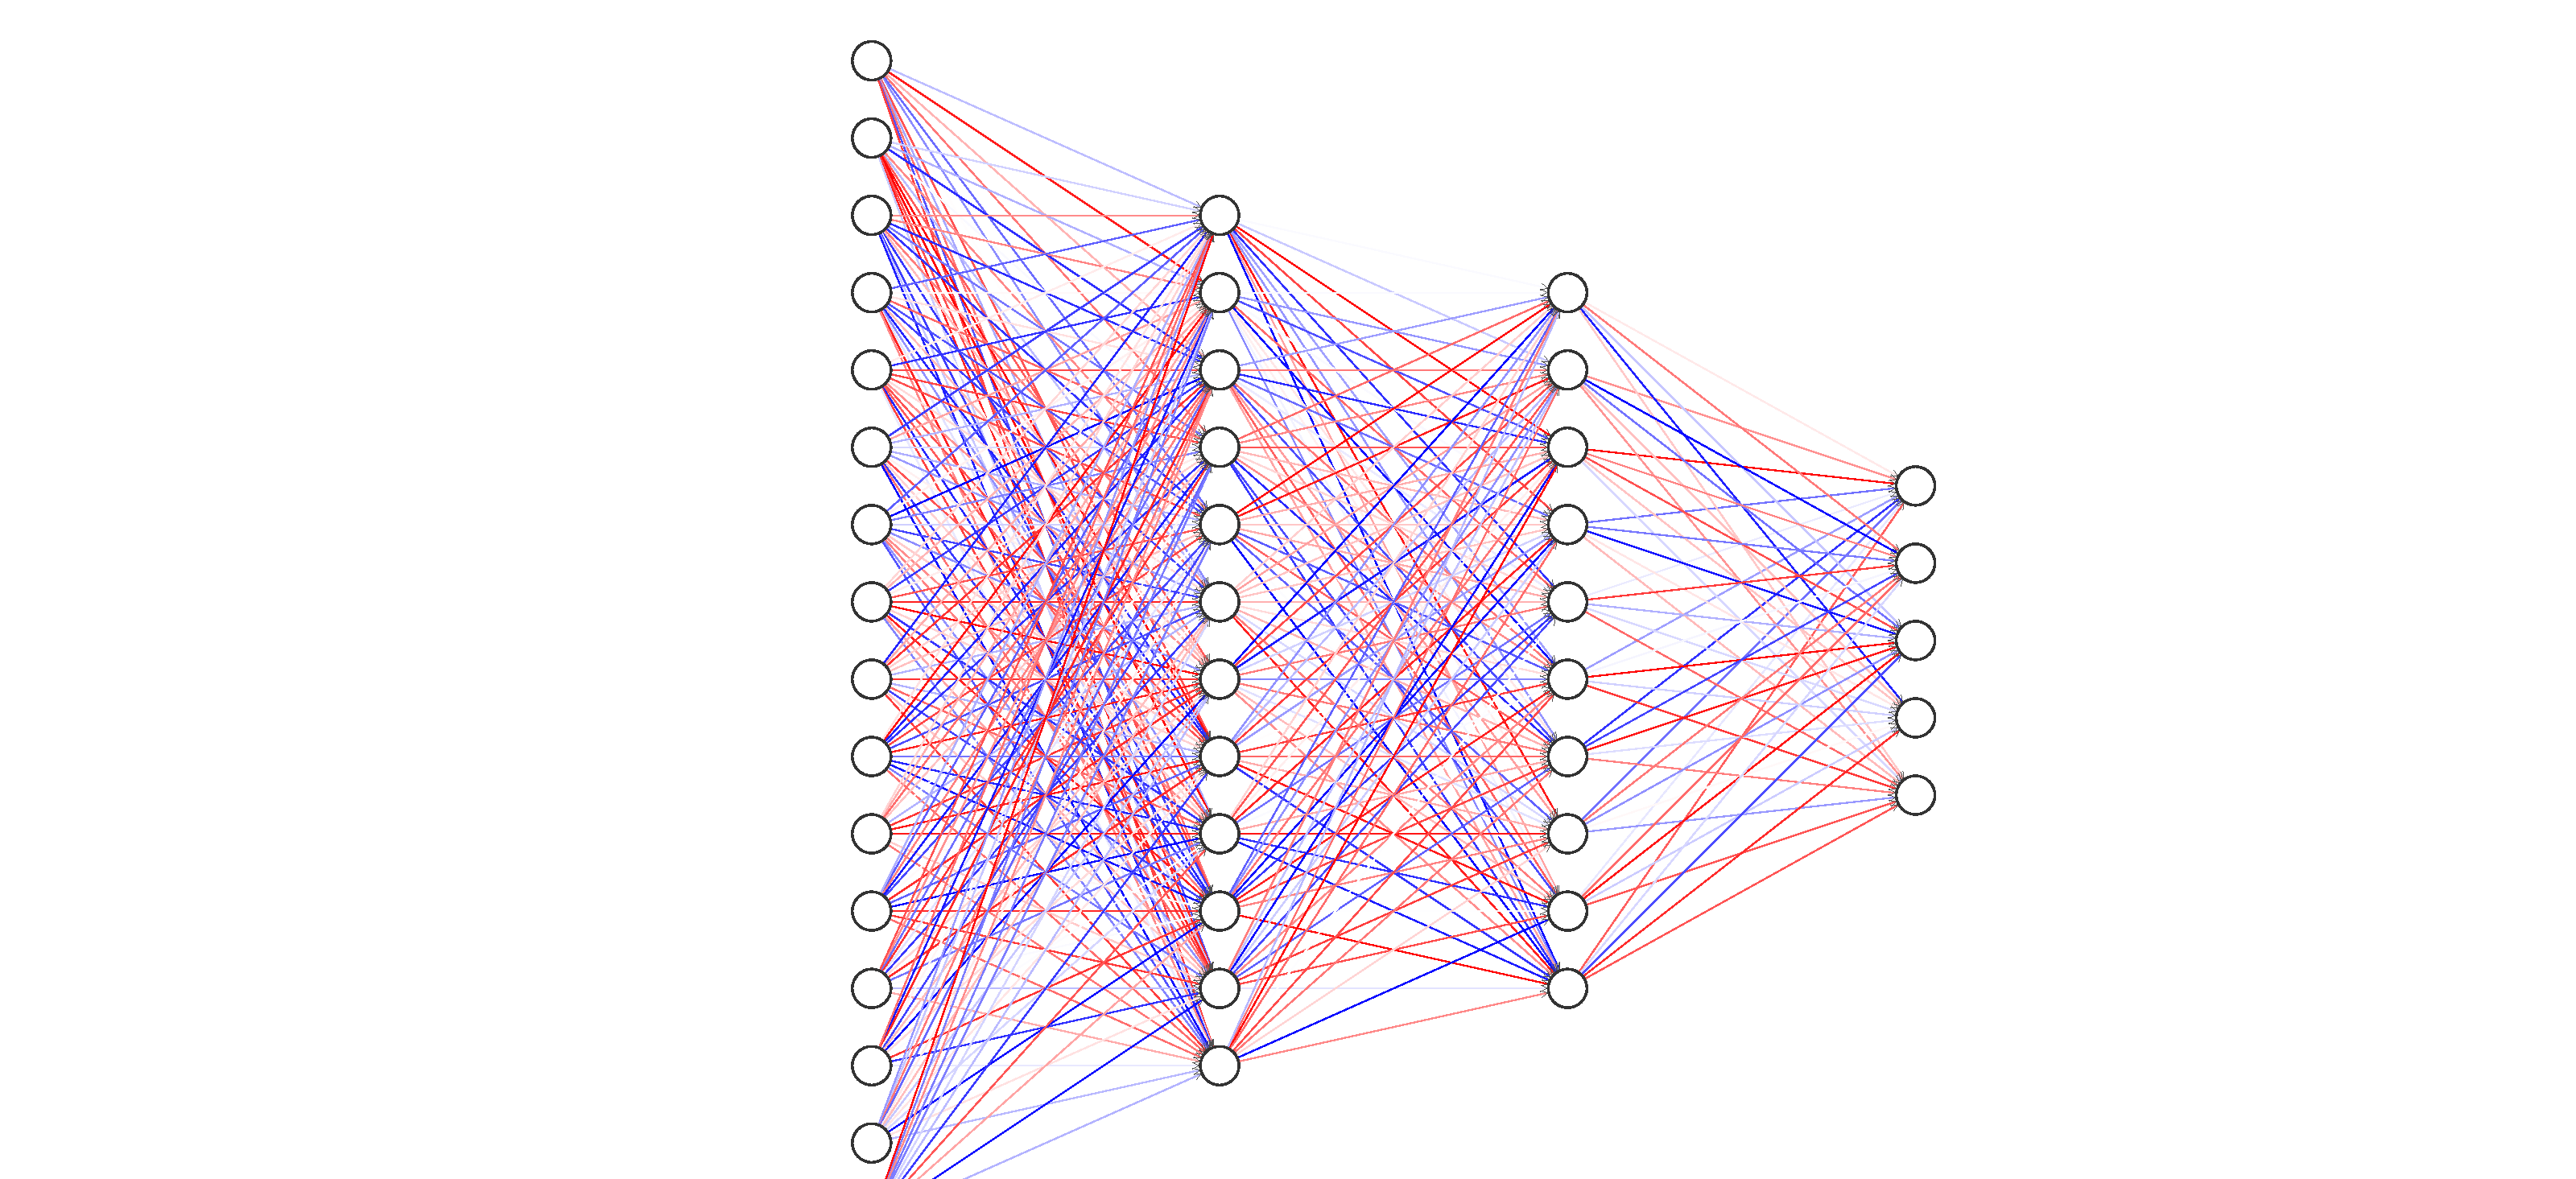
\includegraphics[width=0.5\textwidth]{images/nn}
	\caption{Deep neural network for classification with 5 output classes.}
	\label{fig:dnn0}
\end{figure}

More formally, a feed-forward DNN with $H$ layers, weight matrices $W_1, ..., W_H$, bias vectors $b_1, ..., b_H$ and activation functions $f_1, ..., f_H$ computes a non-linear function \cite{si:dnnhmm}:

$$g_{W, b}(x) := a_H(x) \text{ ,}$$
where, for $h = 1, 2, ..., H$: 

$$a_h(x) = f_h((a_{h-1}(x))^T \cdot W_h + b_h) \text{, and: }$$

$$a_0(x) = x$$
In classification tasks, the last layer activation function is often a softmax function $\sigma$, which outputs a probability $\hat{p}_j$ for each class $j$, and then the class with the highest probability is considered the predicted one:

$$q = \arg \max_j \hat{p}_j \text{, where: }$$

$$\hat{p}_j = f_H(x)_j = \sigma(x)_j := \frac{e^{x_j}}{\sum_{i=1}^{Q}e^{x_i}}$$

\paragraph{DNN training}
Generally speaking, DNN are trained to minimize a loss function $L(W, b)$ (e.g. mean squared error, mean absolute error or binary cross-entropy), and at each training cycle (so-called epochs), weights $W$ and biases $b$ are updated according to their gradient:

$$\nabla_{W, b}(L) = \Big[\frac{\partial L}{\partial b}, \frac{\partial L}{\partial W}\Big]^T \text{; }$$
while gradients are computed using the backpropagation algorithm \cite{backprogation}, the update rule for the weight based on their value can be done in many different ways, and it's in general considered a model hyperparameter to tune. Two notable and popular examples of optimization algorithms to update the network parameters are Stochastic Gradient Descent (SGD) \cite{sgd} and Adadelta \cite{adadelta}, which were also used to train the models for this work.

In multi-class classification tasks such as SI, the most used loss function is the categorical cross-entropy \cite{si:dnnhmm}:

$$L = \sum_{i=1}^{Q} p_j \log \hat{p}_j \text{, }$$
where $p_j$ is the target probability for class $j$ (usually 1 for right class, 0 otherwise) and $\hat{p}_j$ is the network-predicted probability for target class $j$.









